\chapter{Data-driven UI Creation}
\label{chap:corelogic}

In the previous chapter, we described the design principles that guide the implementation and functionality of the \emph{InterfaceSmith} programming system.
This chapter describes the data-driven UI creation feature of the \emph{InterfaceSmith} programming system, expanding upon the principles described in the previous chapter.

Firstly, we describe the \emph{hole-based approach to creating UI elements}, which allows users to create new UI elements based on existing data dynamically.
After that, we describe the \emph{domain model}, mainly the internal representation of the UI elements and necessary operations on these types.
We then describe mapping the input data types to specific types representing the UI elements.
Lastly, we describe how the system combines the input data and UI elements, provides options for creating and modifying the UI elements, and showcase how .
All code examples shown in this chapter are written in the F\#\cite{fsharp} programming language.

\section{Hole-based UI element creation}
\label{sec:hole-based}
The primary motivation of this approach is to alllow \emph{incremental creation} of the user interface based on concrete data.
Rather than creating UI elements for all data fields at once, we provide the functionality to pick what elements to create while still maintaining the structure of the UI based on the input data.

First, the system analyzes the provided data and, based on its structure, creates a UI skeleton containing placeholder types named \emph{holes} that represent potential new UI elements.
Then, the user is provided the option to \emph{fill} these holes with new UI elements that correspond to the particular hole.
The creation process of the UI is then a process of gradually filling the holes with new elements.

The elements are created based on the provided data and its structure; each element corresponds to a data field.
We define the type named \emph{hole} as follows:
\begin{defn}[Hole type definition]
	A \emph{hole} is a placeholder type representing a UI element that is yet to be created despite its existing corresponding data.
	It serves as a temporary stand-in during the incremental construction of a user interface.
\end{defn}

For example, imagine we possess the data shown in Figure~\ref{fig:part-json}, and we wish to create a web application containing a UI element displaying the value of the \emph{Celsius} field.
\begin{figure}[htbp]
	\begin{lstlisting} 
      {
        "Celsius": 0,
        "Farenheit": 0
      }
    \end{lstlisting}
	\caption{Example JSON data}\label{fig:part-json}
\end{figure}
We upload the data to the programming system, and it presents us with the \emph{hole} elements for the \emph{Celsius} and \emph{Farenheit} fields.
Then, we can choose the option to fill the hole corresponding to the \emph{Celsius} field, which creates a new UI element displaying the Celsius's value.
However, we can also create the UI element for the \emph{Farenheit} field anytime while still maintaining that the UI elements' structure corresponds to the data structure.
We can also delete the UI element corresponding to the \emph{Celsius} field, and the system creates the hole again; in other words, we ``dig up'' the element.

We define the \emph{incremental creation process} as a \emph{sequence of operations}.
Each operation is either a \emph{modification} of an existing UI element or a \emph{replacement} of a Hole element with a new UI element based on the corresponding data.
This approach allows the system to perform different tasks after each operation.
These tasks include updating the UI element preview, analyzing the input data, or providing new modification menus and options.

\section{Domain model and Mapping}
\label{sec:types}

In the previous section, we defined the hole-based UI element creation. To provide this functionality, we must first define the types representing the provided data, the UI elements, and how we create the elements corresponding to specific data fields.
In this section, we describe the types that the system uses to represent the input data and the types used to represent the created UI elements,
as well as define the mapping between the input data and the UI element representation.


\subsection{JSON Type}
\label{sub:json}
The creation process starts by providing \emph{JSON} data to the system.
In order to use this data, we parse it and create an internal representation.
We parse the input data using a library called \citet{simpleJson}.
The library defines a discriminated union type named \emph{JSON}.
This type is the foundation for the Abstract Syntax Tree representation of the JSON data.
We can see the type definition in Program \ref{fig:json}.

Each node represents a JSON value in the input data.
The types of nodes can be divided into two categories:
\begin{itemize}
	\item {\textbf{Collections:} The first category contains types representing a \emph{collection} of other values. This category includes the types \emph{JObject} and \emph{JArray}.
	      We define the two collection types as follows:
	      \begin{itemize}
		      \item \textbf{JObject:} It is based on the JSON Object type and represents a collection of different JSON types. The original ordering of the inner elements is \emph{ignored}.
		      \item \textbf{JArray:} It is based on the JSON List type and represents a collection of JSON values of the \emph{same type and structure}. The original ordering of the inner elements is \emph{preserved}.
	      \end{itemize}
	      }
	\item \textbf{Primitives:} The second category contains types representing data primitives such as numerical values, boolean values,
	      a string of text, or the null value.
\end{itemize}

\begin{listing}[H]
	\caption {JSON type}
	\label{fig:json}
	\begin{lstlisting}
type Json =
    | JNumber of float
    | JString of string
    | JBool of bool
    | JNull
    | JArray of Json list
    | JObject of Map<string, Json>
  \end{lstlisting}
\end{listing}

\subsection{RenderingCode Type}
To facilitate the creation of UI elements based on the JSON type, we define a type named \emph{RenderingCode}.
The \emph{RenderingCode} is a discriminated union type used to represent the UI elements.
Similarly to the JSON type, each case represents a type of an HTML element with a corresponding mapping to the JSON type.
This type is the foundation for the \emph{Abstract Syntax Tree} representation of UI elements.
We can see the type definition in Program~\ref{fig:renderingCode}.
\begin{listing}[htbp]
	\caption {RenderingCode type}
	\label{fig:renderingCode}
	\begin{lstlisting}
type RenderingCode =
    | HtmlElement of 
        tag: Tag * 
        attrs: Attributes * 
        innerValue: InnerValue * 
        eventHandlers: (string * EventHandler) list
    | HtmlList of
        listType: ListType *
        attrs: Attributes *
        itemCodes: RenderingCode list *
        eventHandlers: (string * EventHandler) list
    | HtmlObject of
        objectType: ObjType *
        attrs: Attributes *
        keyOrdering: string list *
        codes: Map<string, RenderingCode> *
        eventHandlers: (string * EventHandler) list
    | Hole of FieldHole
 
  \end{lstlisting}
\end{listing}

\subsubsection{Attributes}
The RenderingCode type, except the case type \emph{Hole}, provides the ability to create and modify custom \emph{Attributes}.
The \emph{Attributes} type represents a collection of key-value pairs representing HTML attributes.
An \emph{Attribute} consists of a \emph{key} of a type \emph{string} and an \emph{value} of a type \emph{InnerValue} whose definition we see in Program~\ref{fig:innerVal-type} and
we can see the type definitions fot the \emph{Attributes} and \emph{Attribute} types in Program~\ref{fig:attrs-type}.
\begin{listing}[H]
	\caption{Attribute and Attributes type definition}
	\label{fig:attrs-type}
	\begin{lstlisting}
type Attribute = {
    Key: string
    Value: InnerValue
    Namespace: string option
}

and Attributes = Attribute list
    \end{lstlisting}
\end{listing}


Each HTML element can contain several associated attributes, and different types of HTML elements allow the use of unique attributes, such as the \emph{type} attribute for the \emph{input} HTML element.
Our editor allows the definition and modification of these attributes through a low-code interface we see in Figure~\ref{fig:attrs-menu}.
The user can create an attribute of a particular key and modify the value by selecting the innerValue case type they wish to use.

\begin{figure}[htbp]
	\begin{center}
		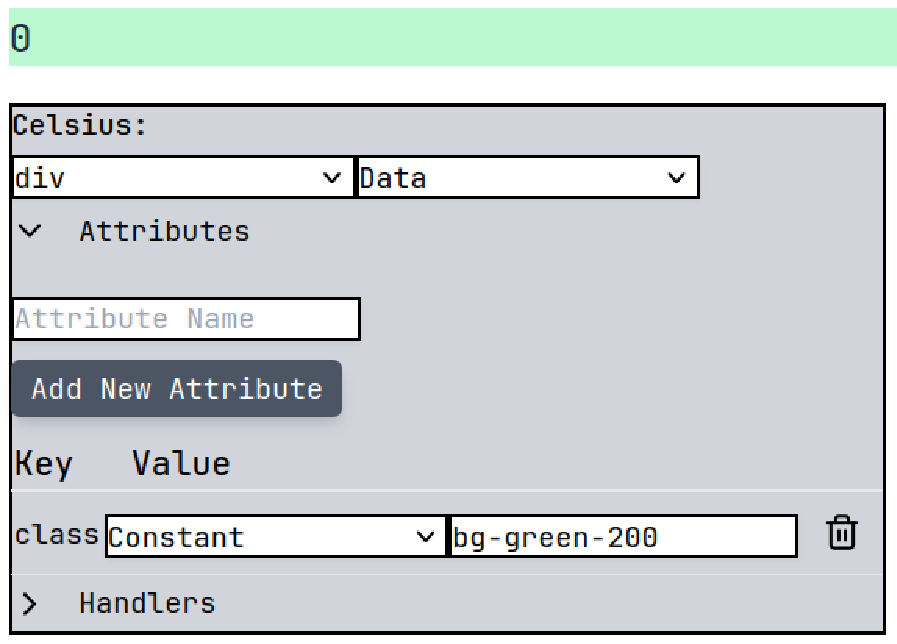
\includegraphics[width=0.8\textwidth]{img/attribute-menu.pdf}
	\end{center}
	\caption{Attribute modification menu for a HtmlElement}\label{fig:attrs-menu}
\end{figure}

\subsubsection{Event Handler}
Each RenderingCode type, except the case type \emph{Hole}, also provides the ability to add custom \emph{event handling} functionality.
A \emph{handler} is a certain function called when when a certain HTML \emph{event} occurs, such as when the element is hovered over or clicked.
Each \emph{EventHandler} consists of the name of a \emph{function} or an \emph{elmish-style message}, depending on how the user wishes to implement custom element behaviour and we see the definition in Program~\ref{fig:handlers-type}.

\begin{listing}[H]
	\caption{EventHandler type definition}
	\label{fig:handlers-type}
	\begin{lstlisting}
and EventHandler =
    | JsHandler of functionName: string
    | MsgHandler of the message: string
  \end{lstlisting}
\end{listing}

We see the menu for assigning the event handling functionality to UI elements in Figure~\ref{fig:handler-menu}.
It provides options to select an \emph{event} and assign a corresponding handler and also indicates wheter the selected handler is a JavaScript function or an elmish-style message.
\begin{figure}[H]
	\begin{center}
		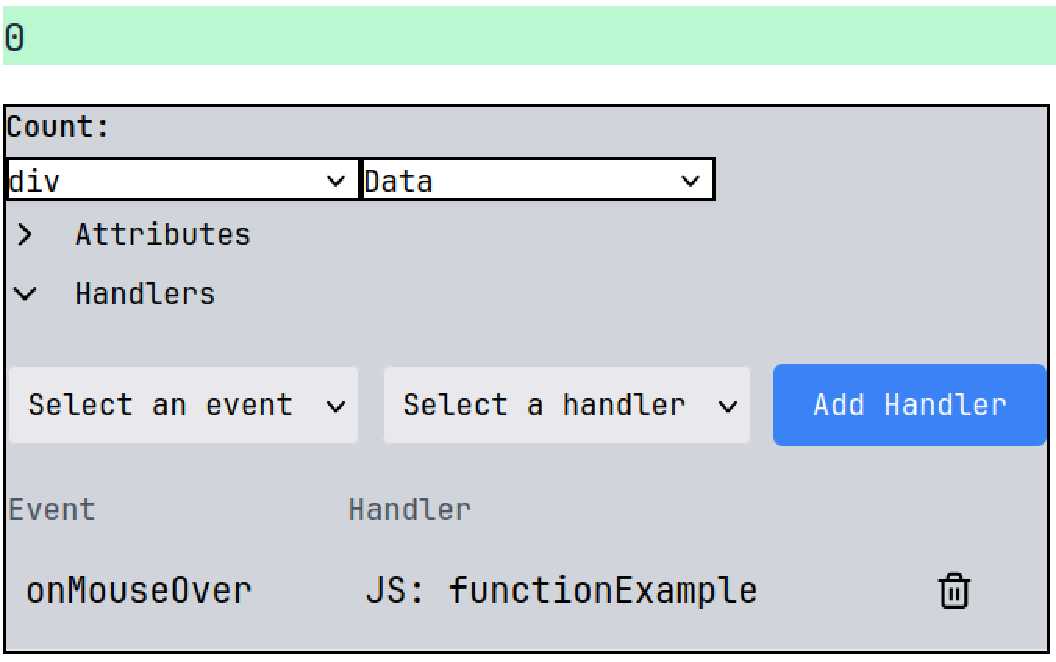
\includegraphics[width=0.8\textwidth]{img/handler-menu.pdf}
	\end{center}
	\caption{EventHandler modification menu for a HtmlElement}\label{fig:handler-menu}
\end{figure}

\subsubsection{Hole}
The \emph{Hole} type represents a placeholder in the UI element structure as defined in Section~\ref{sec:hole-based}, allowing for dynamic element creation.

\subsubsection{HtmlElement}
The \emph{HtmlElement} type represents a single HTML element.
It consists of a tag of a type \emph{Tag}, which denotes the HTML tag (e.g., div, p, span),
the \emph{InnerValue}, which represents the content of the element defined as seen in Program~\ref{fig:innerVal-type}, and the previously defined attributes and event handlers.

The InnerValue's \emph{Data} case type indicates content from the corresponding input JSON value, \emph{Empty} represents an empty element, and \emph{Constant} holds static, developer-defined content.

\begin{listing}[htbp]
	\caption{InnerValue type definition}
	\label{fig:innerVal-type}
	\begin{lstlisting}
type InnerValue =
    | Data
    | Constant of string
    | Empty
    \end{lstlisting}
\end{listing}

\subsubsection{HtmlList}
The \emph{HtmlList} type represents a collection of HTML elements of the \emph{same type and structure} corresponding to JSON arrays.
It consists of a \emph{listType}, which specifies the list type (e.g., unordered, ordered), and we define it as a simple discriminated union type, \emph{itemCodes} is a collection of RenderingCode elements representing the list's contents,
previously defined attributes, and event handlers.
As we assume that the list consists of elements of the same type and structure, when one list element is modified, we can apply these modifications to all remaining elements.

\subsubsection{HtmlObject}
The \emph{HtmlObject} type represents a collection of \emph{diverse} HTML elements derived from a JSON object.
It consists of an \emph{objectType}, which defines the type of the object (e.g., div, span, section) and is defined as a simple discriminated union,
\emph{elements}, which is a list of RenderingCode elements representing the object's contents, and the previously defined attributes and event handlers.

\subsection{Data Mapping: JSON to RenderingCode}
\label{sec:mapping}
Transforming JSON data into UI elements requires systematic mapping between JSON and RenderingCode types.
This mapping forms the core of our UI generation system, allowing us to convert arbitrary JSON input into a structured representation of UI elements.
Each JSON type has a corresponding representation in RenderingCode:
\begin{itemize}
	\item JObject maps to HtmlObject
	\item JArray maps to HtmlList
	\item JNull, JString, JNumber, and JBool map to HtmlElement
\end{itemize}

The \emph{incremental creation process} described in Section~\ref{sec:hole-based} involves dynamically creating replaceable \emph{Hole} elements.
We perform this creation lazily and incorporate it into the mapping process.
A \emph{Hole} element is created for each inner element of the collection types described in Section~\ref{sub:json}.

We call this mapping process the \emph{recognition} of the JSON value and define the mapping function named \emph{recognizeJson} in Program~\ref{fig:recognizeJson}.

\begin{listing}[H]
	\caption {JSON to RenderingCode mapping}
	\label{fig:recognizeJson}
	\begin{lstlisting}
let recognizeJson (json) =
    match json with
    | JArray array -> 
        //create a hole for each element of the array
        HtmlList containing the holes as elements
    | JObject obj ->
        //create a Hole for each element of the object 
        HtmlObject containing the holes as elements
    | JNull -> Hole(UnNamed)
    | _ -> HtmlElement 
  \end{lstlisting}
\end{listing}

\section{Incremental Creation Process}
\label{sec:creation}
We described the \emph{incremental creation process} briefly in Section~\ref{sec:hole-based} as a sequence of operations.
In this Section, we extend this description and define the previously described operations in greater detail.
We divide the operations into two categories:
\begin{itemize}
	\item \textbf{User operations:} Operations performed by the user such as element creation, element modification, and providing data to the system.
	      User operations are performed through the provided GUI.
	\item \textbf{System operations:} Operations performed by the system in reaction to the User operations.
	      These operations include creating new RenderingCode elements, analyzing newly visited JSON values, modifying AST, rendering menus, and previewing elements.
\end{itemize}
This categorization allows us to divide the functionality and responsibilities of the system between different parts of the application.
For example, the GUI portion of the application is mainly responsible for accepting User operations, whereas other modules can implement different System operations.

\subsection{Hole Replacement and Modification}

User operations require finding a specific node inside the RenderingCode AST during the creation process.
We define a dynamically generated \emph{Path} for all nodes during the traversal process to find this specific node.
The \emph{Path} is a sequence of indices unique to every node in the AST.

\begin{listing}[htbp]
	\caption {Example RenderingCode AST with corresponding paths}
	\label{fig:paths}
	\begin{lstlisting}
  HtmlObject(ObjType.Div, [],["key1";"key2"], [ //Path: []
      HtmlElement(Tags.div,[], InnerValue.Empty, []) //Path: [0]
      HtmlList(ListType.UnorderedList,[], [ //Path: [1]
          HtmlElement(Li, [], Constant "Item 1", []) //Path: [1,0]
          HtmlElement(Li, [], Constant "Item 2", []) //Path: [1,1]
        ], [])
    ], [])
  \end{lstlisting}
\end{listing}

We can see the different paths for each element in Program~\ref{fig:paths}, which shows an example of RenderingCode AST.
The example AST consists of a root node of a type HtmlObject and elements contained within it.
We see that the root node has an empty path.
Then, we append the position of each element inside the collection to the Path.
This allows us to traverse the AST based on the specified Path and find the correct element using a recursive search function.

Using the dynamically created paths, we can replace a RenderingCode by following its specified Path through the RenderingCode AST.
We define a recursive function named \emph{replace} which navigates the AST using the provided path to locate and replace a specific element with a new one.
We can see a description of the potential implementation in Program~\ref{fig:replace}.

\begin{listing}[htbp]
	\caption {A function used to replace a RenderingCode inside the RenderingCode AST}
	\label{fig:replace}
	\begin{lstlisting}
let rec replace 
  (path: int list) 
  (replacementCode: RenderingCode) 
  (currentCode: RenderingCode) =
  match path with
  | [] -> replacementElement
  | head :: tail ->
      match currentCode with
      | HtmlList ->
          // recursively call the function on a collection element with the index equal to head 
          // return new HtmlList
      | HtmlObject ->
          // recursively call the function on an element with 
          // the key located inside the keys collection, that has index equal to head
          // return new HtmlObject
      | _ -> currentCode // remaining path, but the current element is not a collection -> no changes to the RenderingCode
  \end{lstlisting}
\end{listing}

The User operations such as replacing a Hole with a new RenderingCode or modification of an existing RenderingCode correspond to a specific usage of the replace function.

\subsection{Traversal}
\label{sec:traversal}
An essential aspect of the creation process is how the system processes the JSON AST and helps users build the RenderingCode AST.
The process involves traversing both the JSON and RenderingCode ASTs simultaneously.
Our system can perform this simultaneous traversal because we create the RenderingCode AST based on the structure of the existing JSON AST.
This allows the system to dynamically create Hole elements for direct descendants of existing RenderingCode elements for which corresponding data exists, but the elements have not yet been created.

Another way to look at this process is that the RenderingCode AST is guiding our traversal, while the JSON AST inspires the structure of the RenderingCode AST.
The traversal begins from the roots of the ASTs, and we traverse the trees recursively.
Based on the type of the visited RenderingCode node and the mapping described in Section~\ref{sec:mapping}, we can perform different operations:
\begin{itemize}
	\item \textbf{HtmlElement:} The node is of type HtmlElement, which maps to a primitive JSON value. This means the JSON value has no descendants, and we can end the traversal.
	      The system then performs the operations of displaying a preview of the HtmlElement and a modification menu.
	\item \textbf{Hole:} The node is of type Hole, meaning the JSON value was visited before, but the user has not created the corresponding RenderingCode.
	      The presence of a Hole element also means that we cannot visit the potential descendants, and we can stop the traversal.
	      The system displays a menu to add a new element corresponding to the JSON value.

	\item \textbf{HtmlList and HtmlObject:} When the node represents a \emph{Collection} type of type HtmlList or HtmlObject, we recursively traverse all its descendants.
	      The system displays a modification menu for the element and continues the traversal.
\end{itemize}

After every User operation, the system performs this traversal to update the element preview and modification menus to reflect changes made to the RenderingCode AST.

\subsection{Combining RenderingCode and JSON data}
Once the RenderingCode AST is created, the system needs to combine the RenderingCode elements with the data from the JSON AST.
We use \emph{Structural referencing} to combine a RenderingCode element with the corresponding JSON value.
By Structural referencing we describe a process where a RenderingCode with a specific assigned Path is combined with a JSON value with the same Path.
We can do this easily, as the structure of the RenderingCode AST mirrors that of the JSON AST.
Thanks to the approach of Structural referencing, we can perform this process during our previously described traversal in Section~\ref{sec:traversal}.

\subsection{Creation of a single RenderingCode}

Creating a single RenderingCode element consists of multiple System operations and a single User operation.
We can see the sequence of operations in Figure~\ref{fig:element-creation}.

The process starts when the system visits a previously unvisited node of the JSON AST during the traversal described in Section~\ref{sec:traversal}.
The system automatically creates a corresponding Hole element and adds it to the RenderingCode AST.
Then, the system displays a menu to the user, allowing them to replace the Hole element with a RenderingCode based on the JSON value.
After the user chooses to add the new RenderingCode element, the system uses the previously defined \emph{recognizeJson} function to create the new element based on the corresponding JSON value.
Following that, the system uses the \emph{replace} function to replace the existing Hole element at the specified path with the newly created RenderingCode.
Lastly, the system traverses the modified RenderingCode AST and JSON AST as described in Section~\ref{sec:traversal} and performs operations such as displaying modification menus and element preview.

\begin{figure}[H]
	\centering
	\begin{tikzpicture}[node distance=1.5cm and 1.5cm, auto,
			user/.style={rectangle, draw=black, thick, fill=yellow!20,
					text width=7em, text centered, rounded corners, minimum height=3em},
			system/.style={rectangle, draw=black, thick, fill=blue!20,
					text width=7em, text centered, rounded corners, minimum height=3em},
			legend/.style={rectangle, draw=black, thin, fill=white,
					text width=4em, text centered,rounded corners, minimum height=2em, font=\footnotesize},
			line/.style={draw, thick, -stealth', shorten >=2pt, shorten <=2pt}]

		% Define nodes
		\node [system] (concrete) {New JSON value visited};
		\node [system, right=of concrete] (hole) {Create a Hole};
		\node [system, right=of hole] (holemenu) {Display Hole Menu};
		\node [user, below=of holemenu] (replace) {Replace Hole};
		\node [system, left=of replace] (recognize) {Create new RenderingCode based on JSON value};
		\node [system, left=of recognize] (update) {Update AST with new RenderingCode};
		\node [system,  below=of update] (final) {Traverse the Newly modified RenderingCode AST};

		% Draw connections
		\path [line] (concrete) -- (hole);
		\path [line] (hole) -- (holemenu);
		\path [line] (holemenu) -- (replace);
		\path [line] (replace) -- (recognize);
		\path [line] (recognize) -- (update);
		\path [line] (update) -- (final);
		% Add step numbers and labels
		\foreach [count=\i] \n/\l in {concrete/System, hole/System, holemenu/System, replace/User,recognize/System, update/System,  final/System}
			{
				\node[font=\small, above left, text=black] at (\n.north west) {\i};
				\node[font=\tiny, below right, text=black] at (\n.south east) {\l};
			}

		% Compact Legend
		\node[legend, fill=yellow!20,  right=1cm of final] (user_legend) {User Operation};
		\node[legend, fill=blue!20, right=0.5cm of user_legend] (system_legend) {System Operation};

	\end{tikzpicture}
	\caption{Single RenderingCode Creation Process}
	\label{fig:element-creation}
\end{figure}

\subsection{Simple TODO list UI creation}

As we defined the necessary
We see the steps of the entire process in Figure~\ref{fig:simple-todo-steps}.

The process starts by uploading the JSON data displayed in Figure~\ref{fig:simple-todo-json} to the system.
The system analyzes it and creates a UI skeleton displaying the hole menus for the \emph{title} and \emph{tasks} fields.
We then click on the button to replace the \emph{hole} corresponding to the title field. The system automatically creates a new HtmlElement, displaying its preview and a modification menu.
We repeat the process for the tasks field, and the system creates a new HtmlElement and a hole for the list elements.
As described in the previous section, we assume the list contains elements of the same type and structure, allowing the system to show modification menus only for the first list element. All changes made to it affect all other elements.
After replacing the modification hole, the system finally creates the final HTML elements for each element of the list, and modification menus are displayed for all RenderingCode elements.
Finally, we click the \emph{Toggle Options} button and see the preview of the created elements without the modification menus present.

\begin{figure}[H]
	\centering
	\begin{lstlisting} 
      {
        "title": "TODO list",
        "tasks": [
            {
            "task": "Complete project proposal"
            },
            {
            "task": "Prepare presentation slides"
            },
            {
            "task": "Send meeting agenda to team"
            }
        ]
      }
    \end{lstlisting}
	\caption{Example TODO list JSON data}\label{fig:simple-todo-json}
\end{figure}


\begin{figure}[p]
	\vspace{-1cm}
	\centering

	\begin{tikzpicture}[
			node distance=1.5cm and 2cm, % Adjust spacing
			auto,
			line/.style={draw, thick, -stealth', shorten >=2pt, shorten <=2pt},
			stepnode/.style={rectangle, draw=black, thick, fill=white, text centered, text width=10em, minimum height=4em}
		]
		% Define nodes with smaller, proportional image sizes
		\node (json) {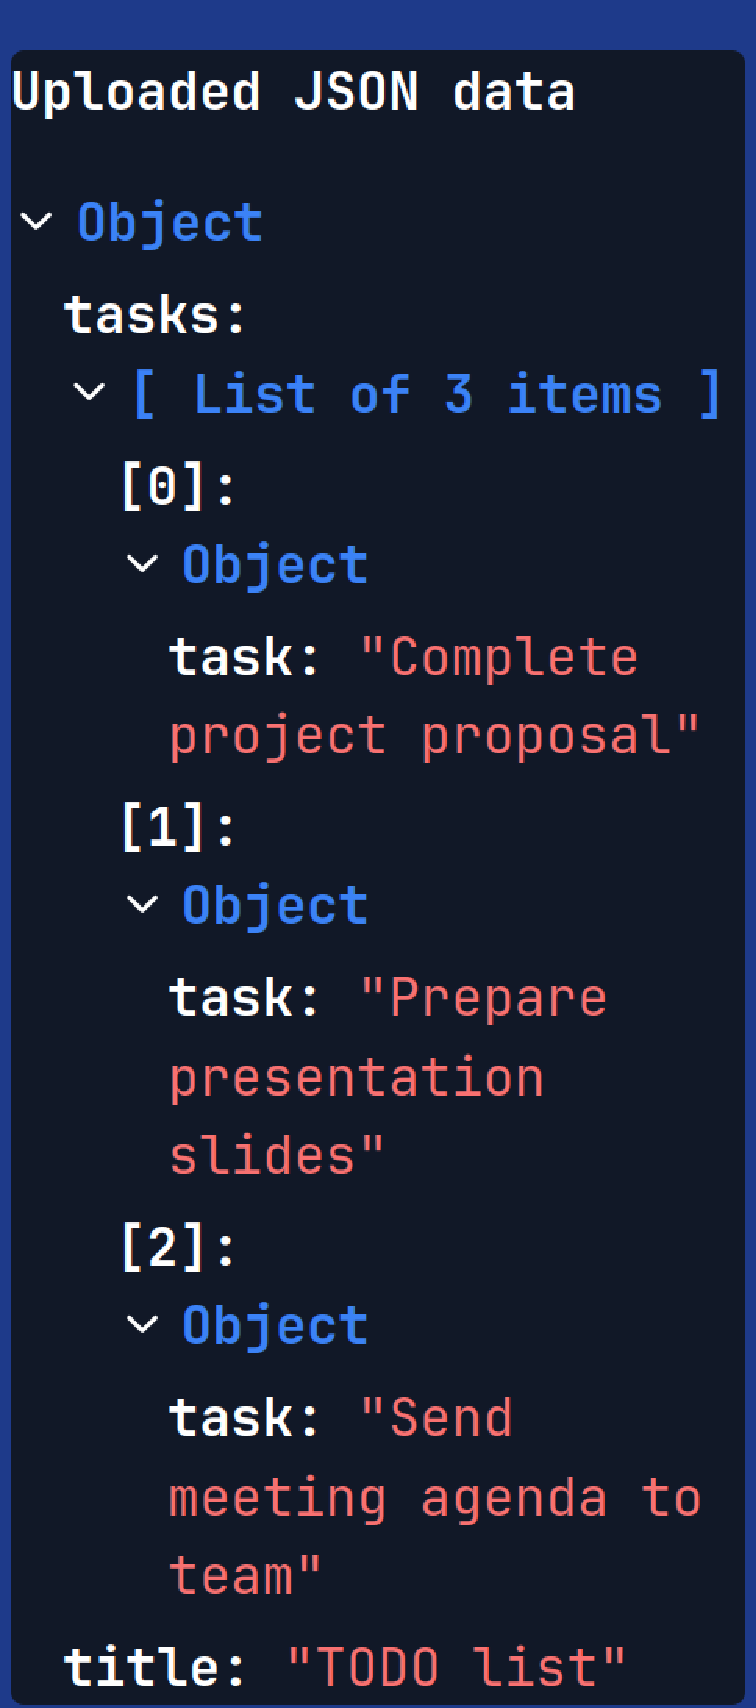
\includegraphics[width=0.2\textwidth]{img/simple-todo-json.pdf}};
		\node [right=of json] (todo1) {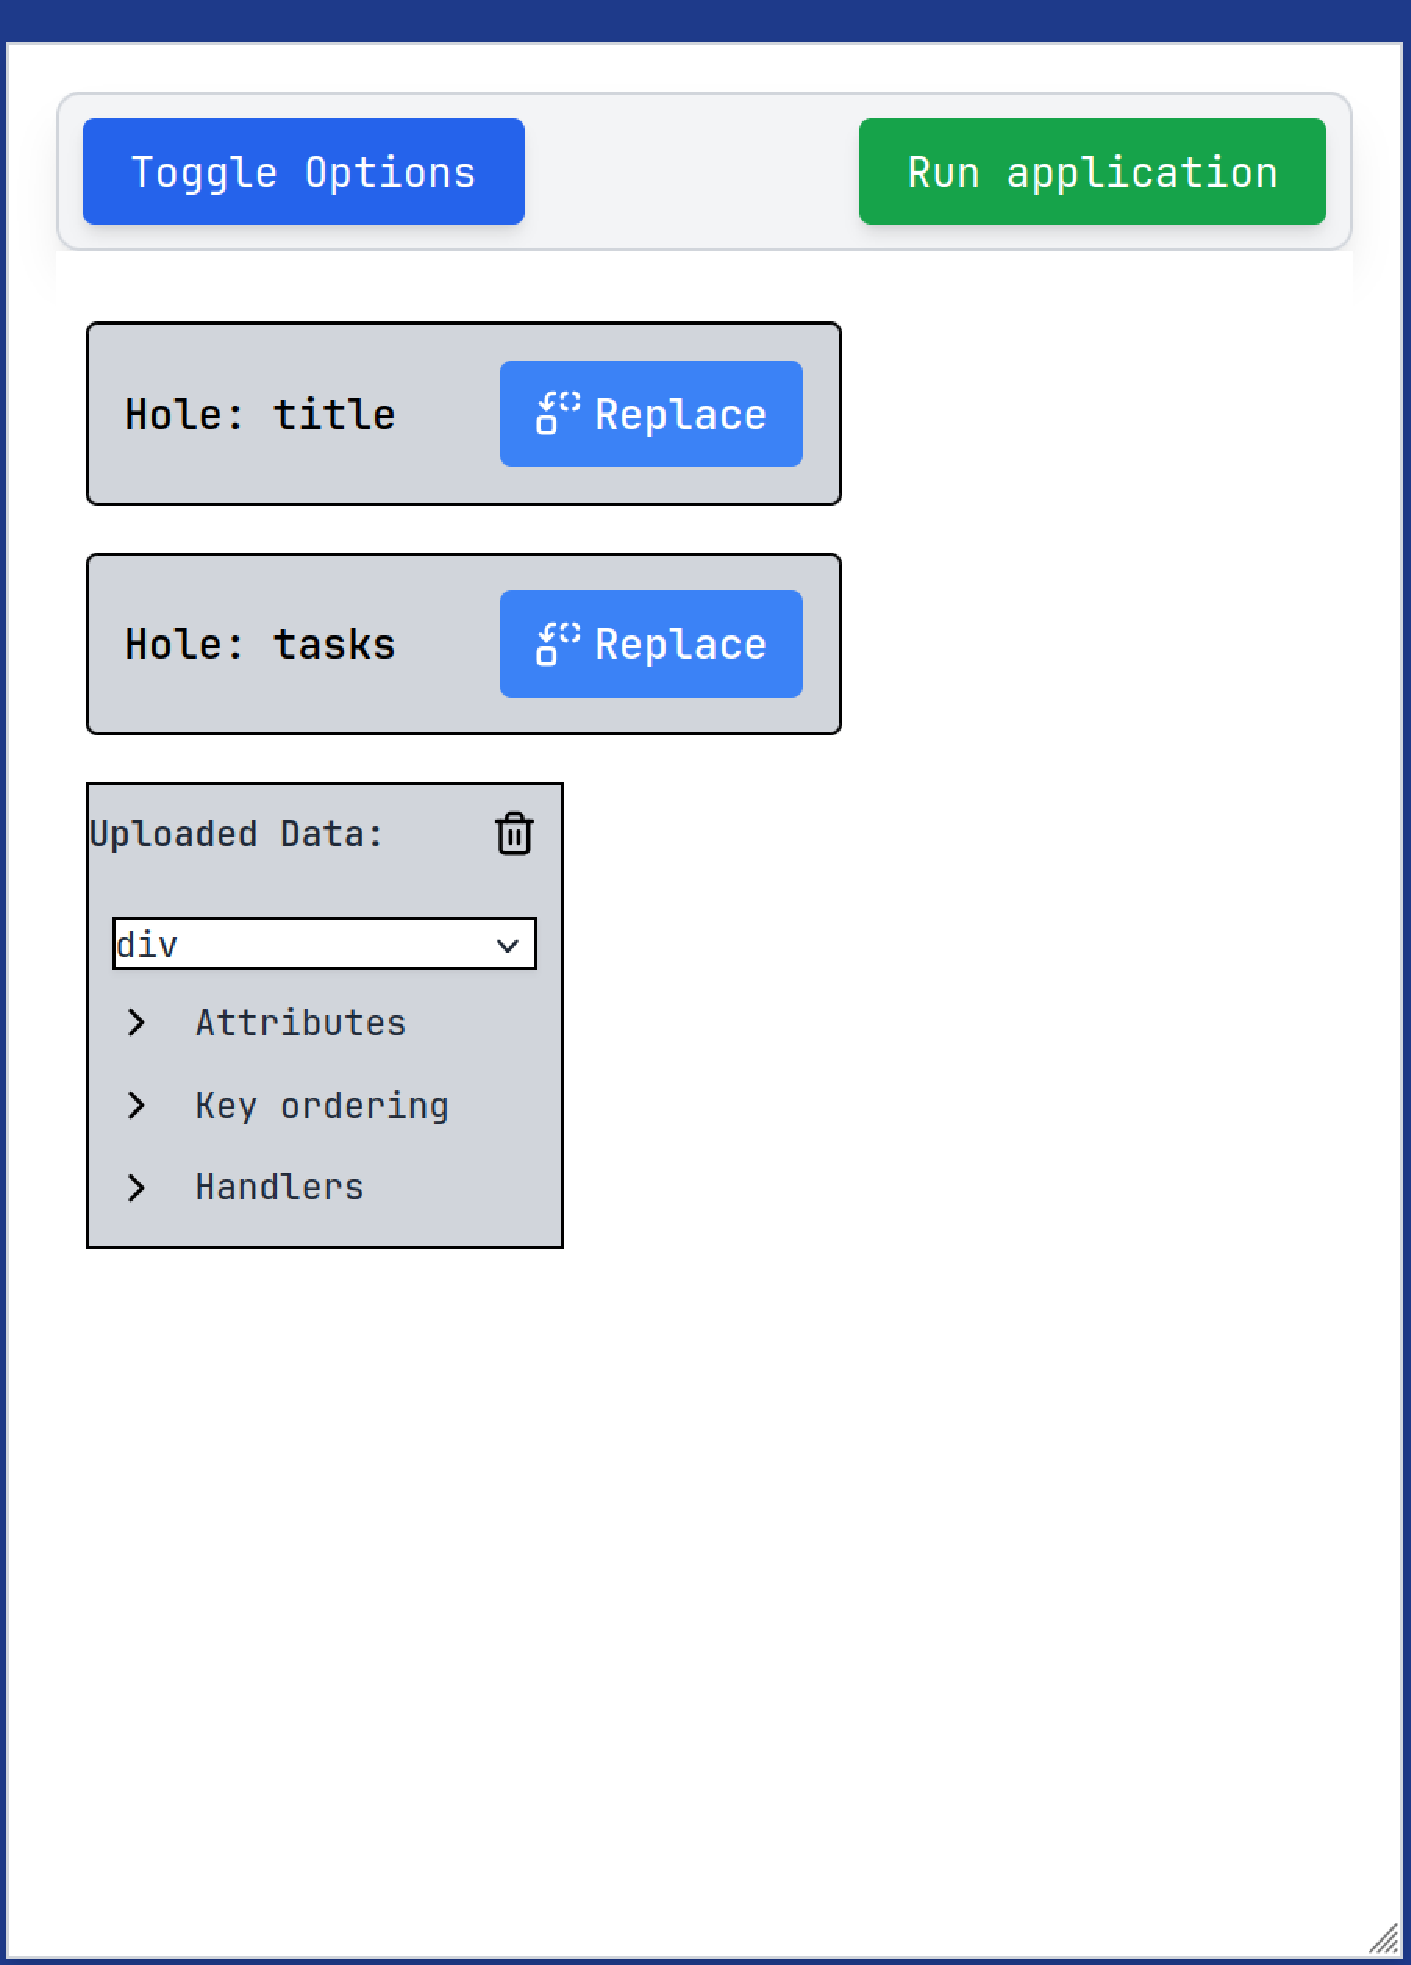
\includegraphics[width=0.35\textwidth]{img/todo-simple-1.pdf}};
		\node [below=of json] (todo2) {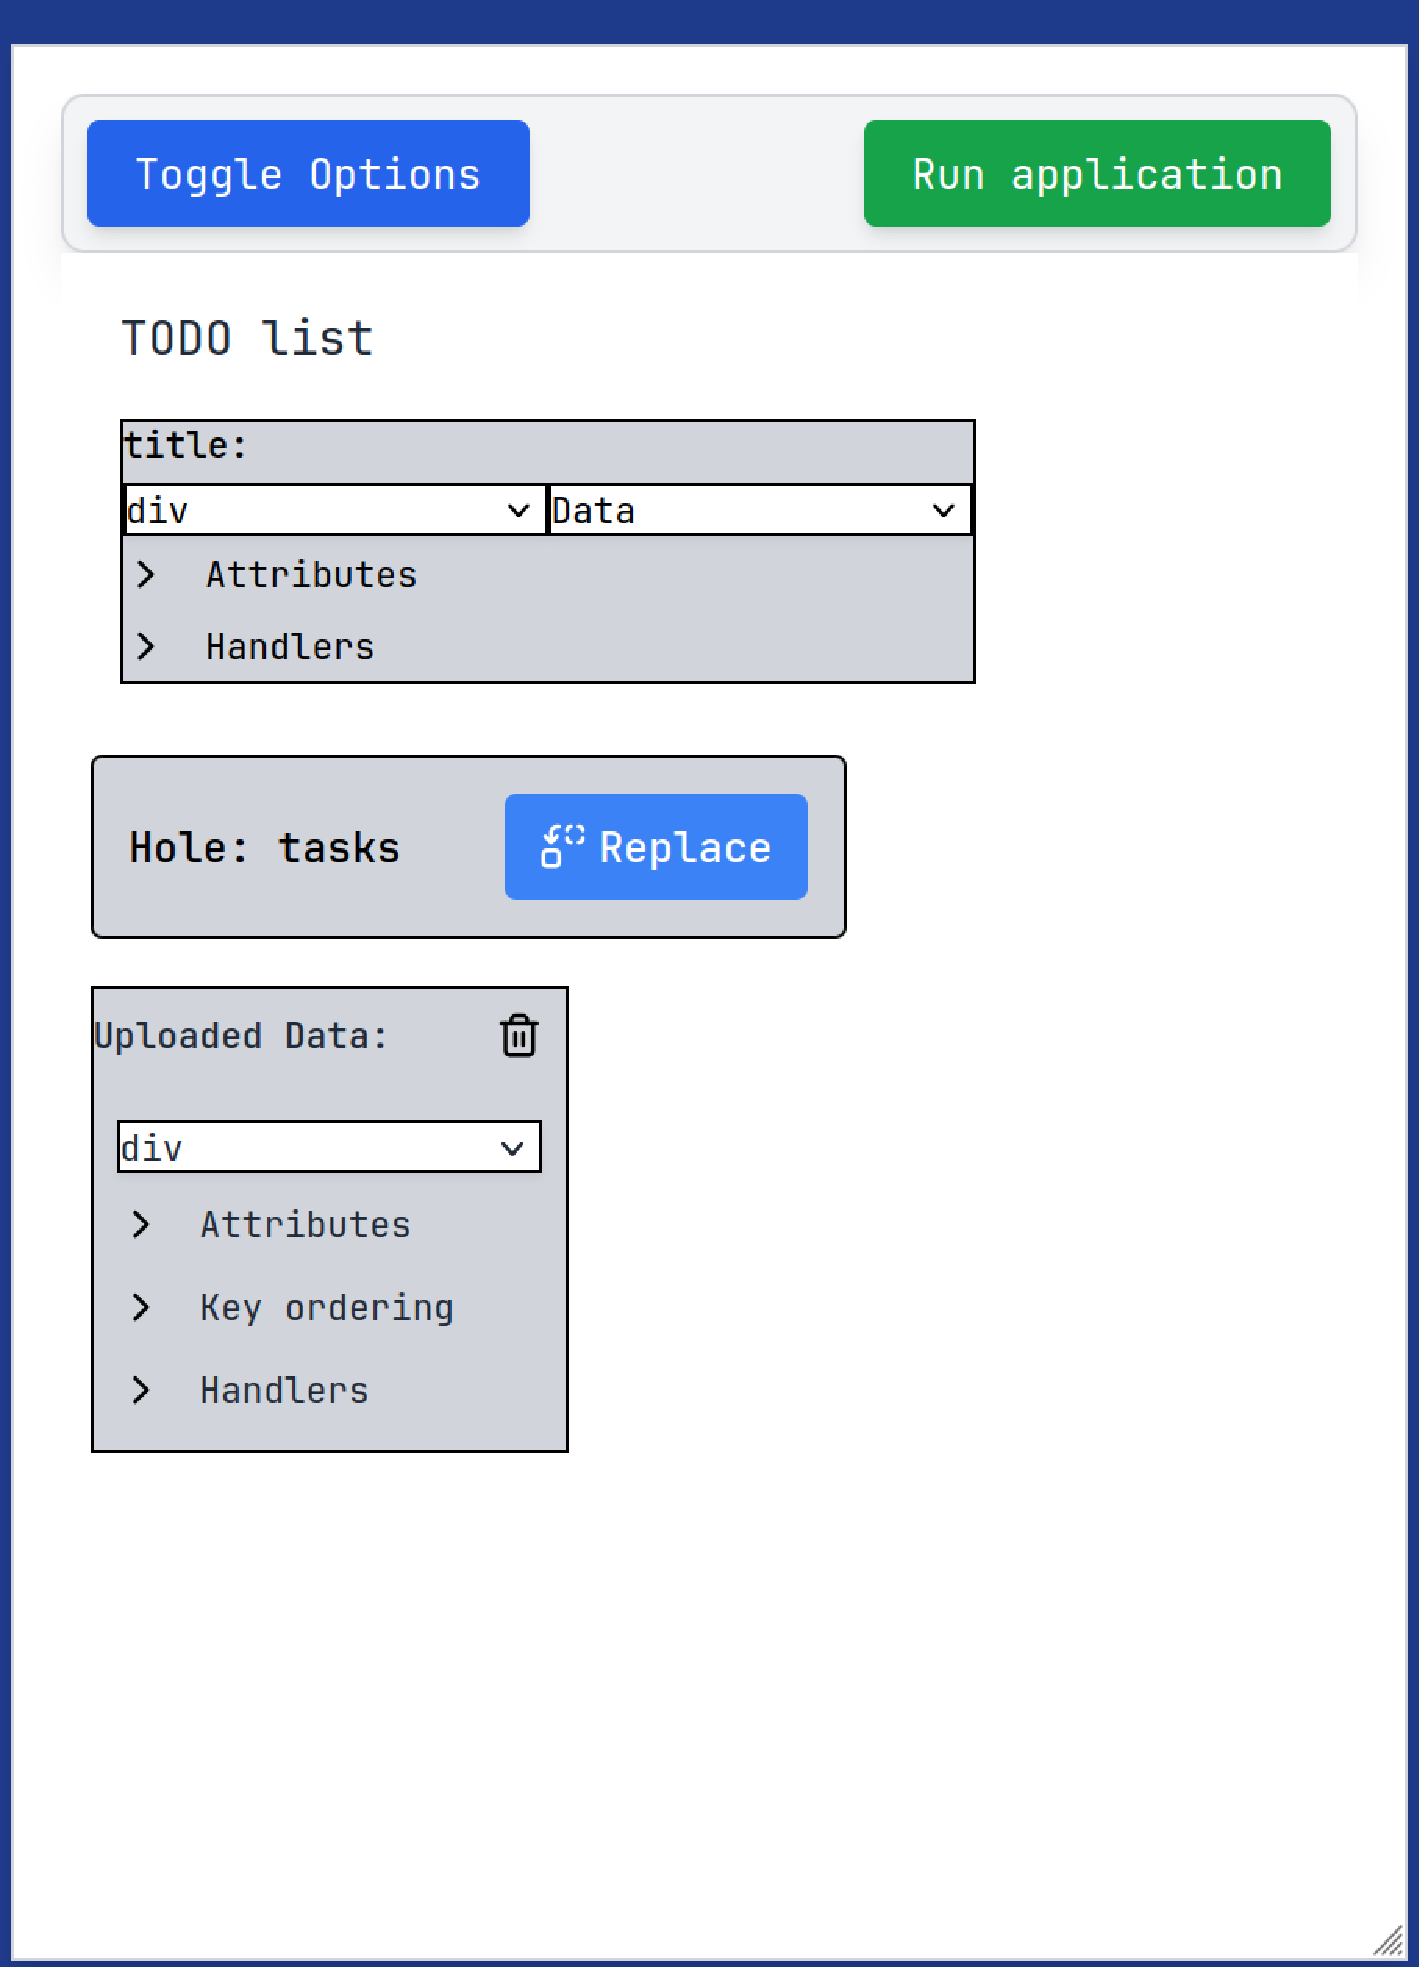
\includegraphics[width=0.35\textwidth]{img/todo-simple-2.pdf}};
		\node [right=of todo2] (todo3) {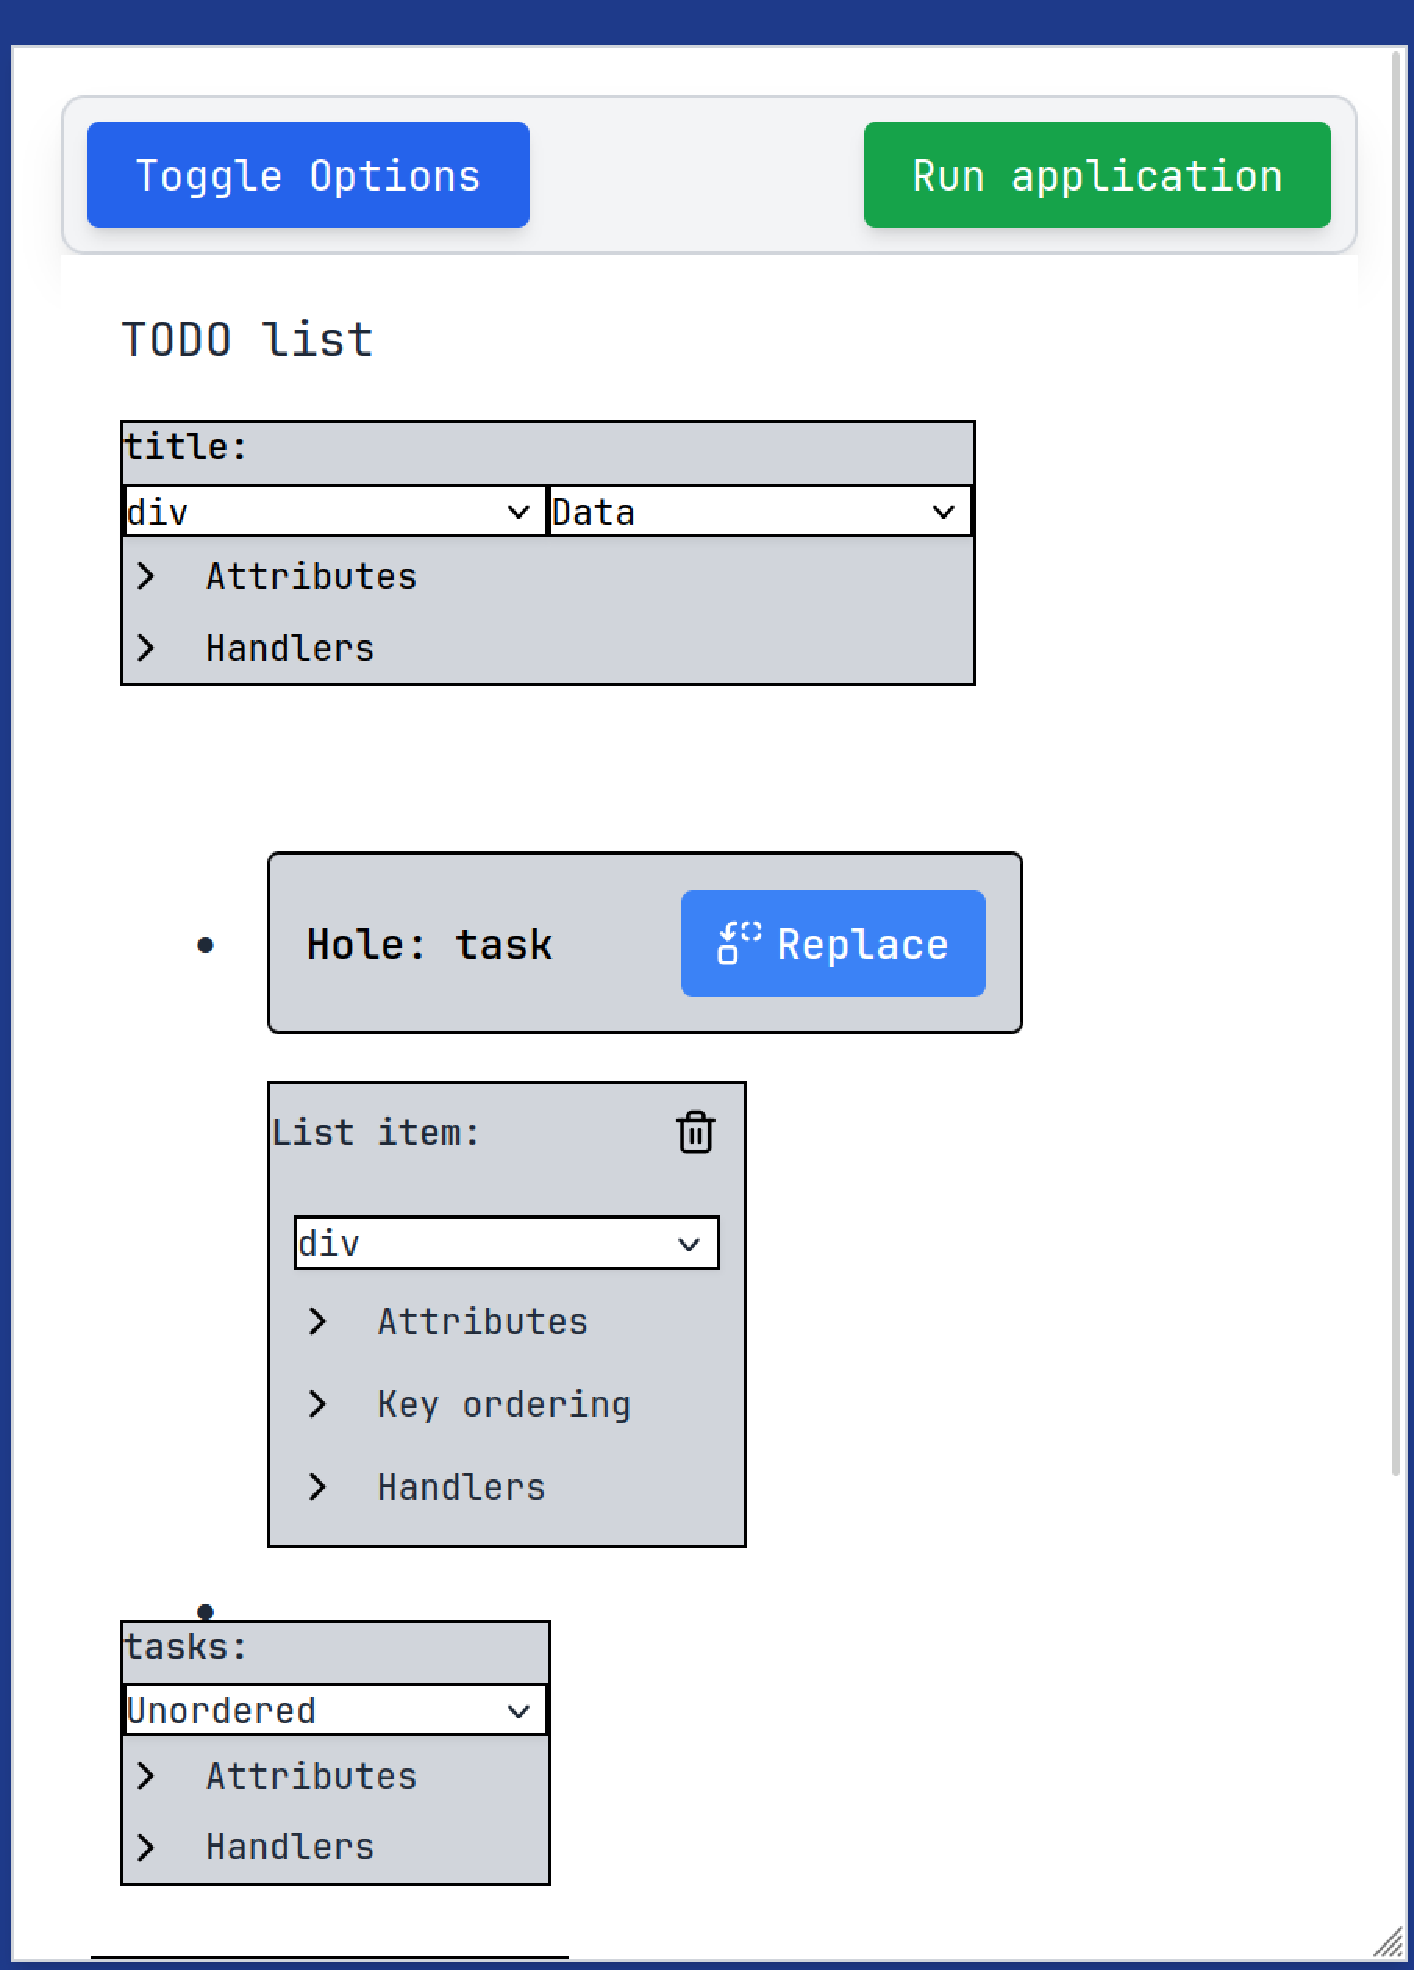
\includegraphics[width=0.35\textwidth]{img/todo-simple-4.pdf}};
		\node [below=of todo2] (todo4) {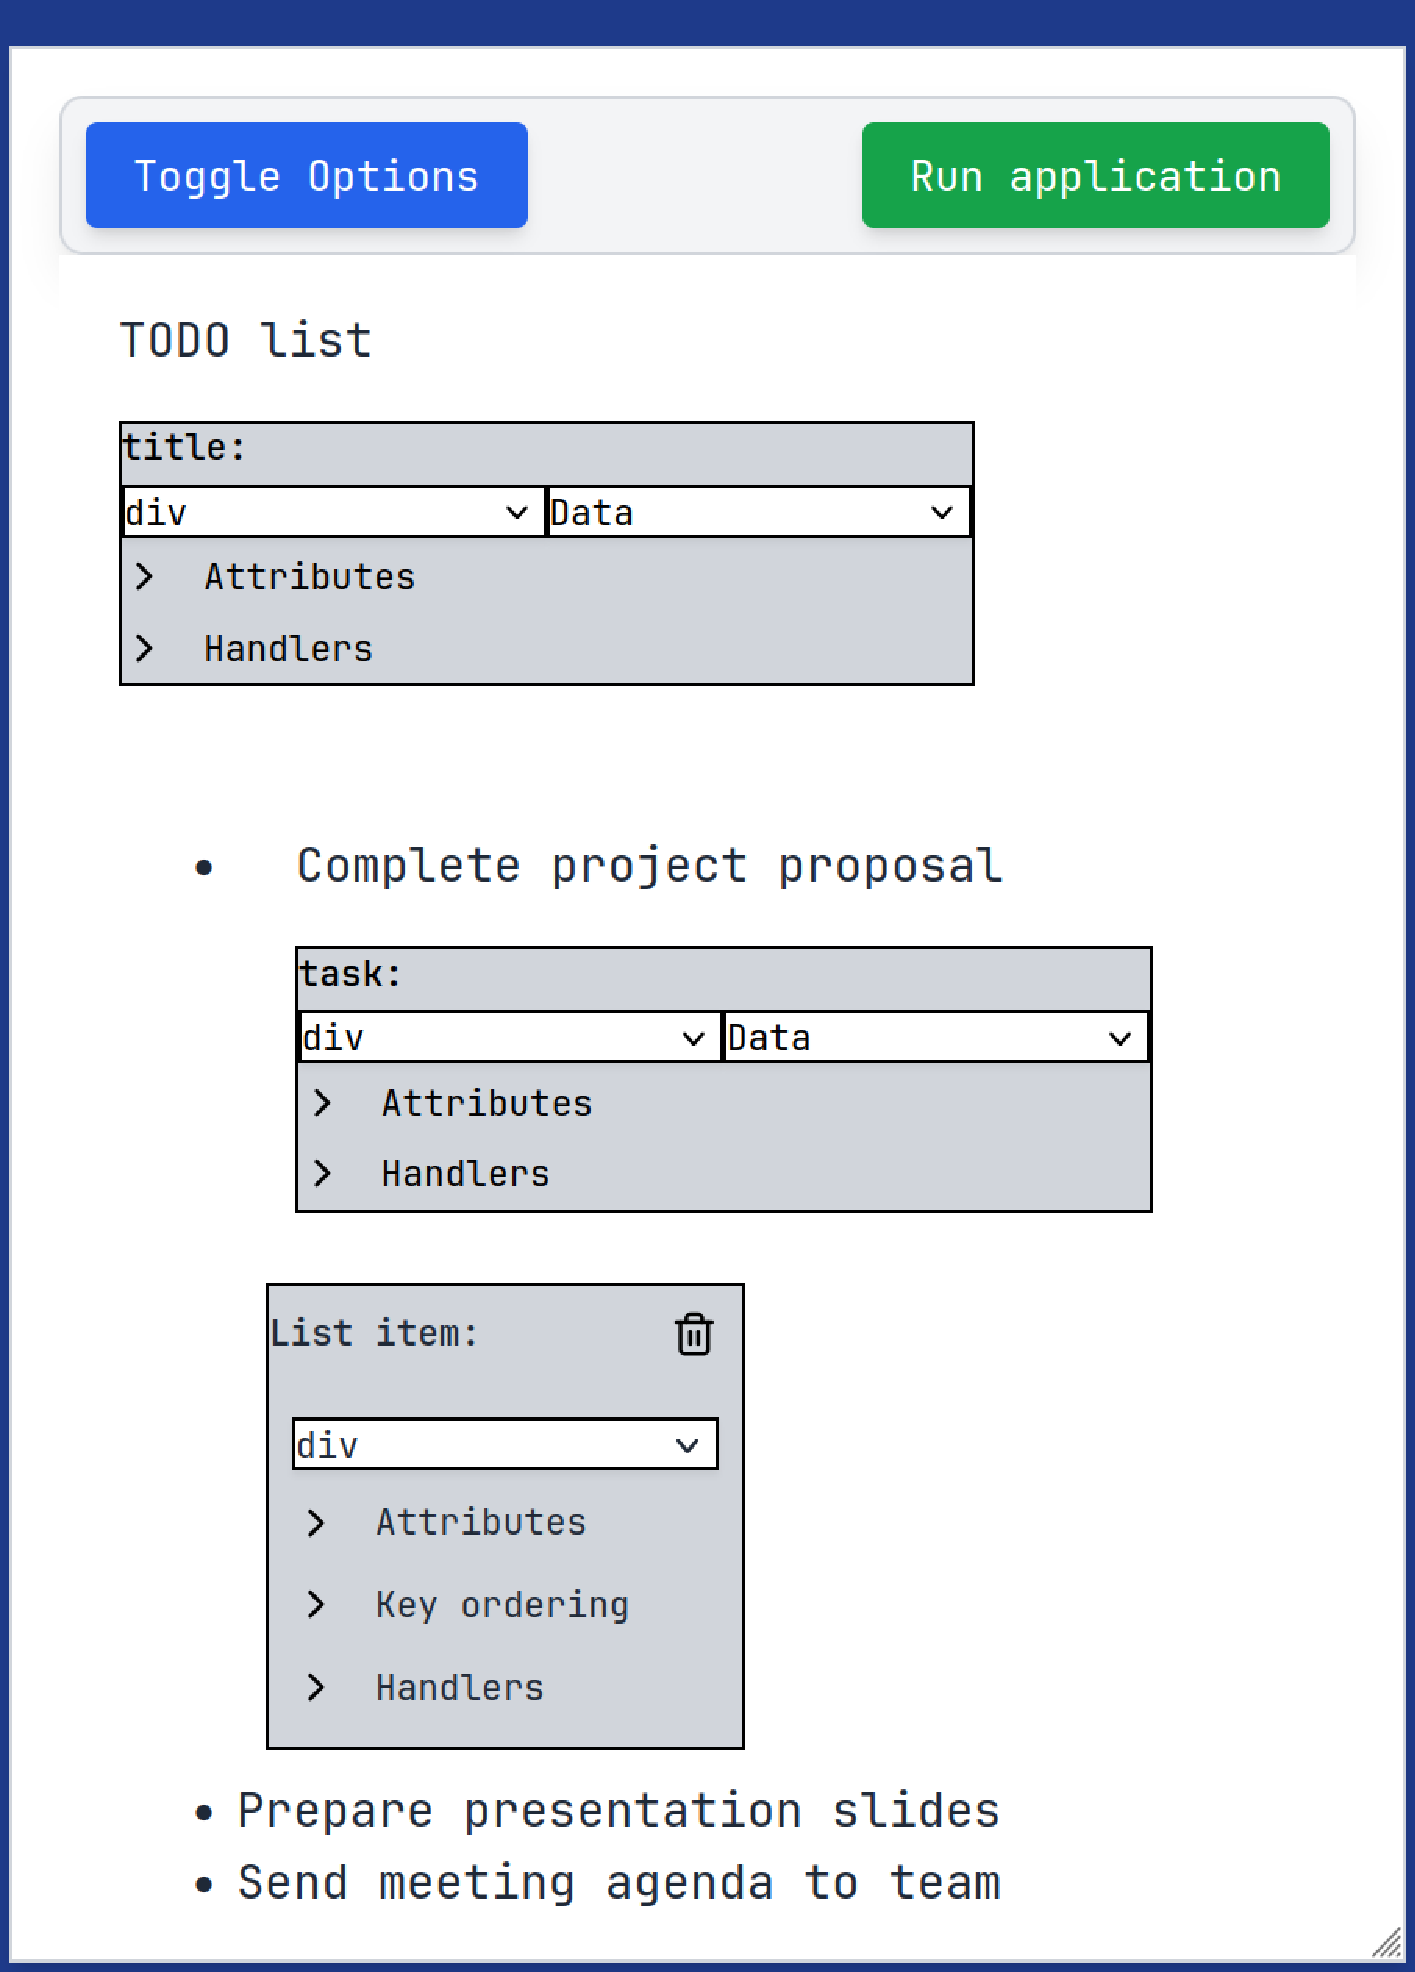
\includegraphics[width=0.35\textwidth]{img/todo-simple-5.pdf}};
		\node [right=of todo4] (todo5) {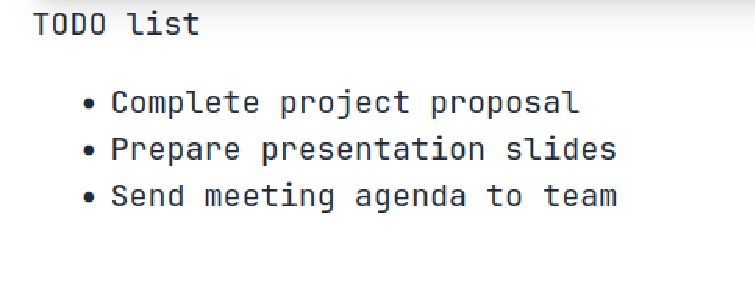
\includegraphics[width=0.35\textwidth]{img/todo-simple-6.pdf}};

		% Draw arrows between nodes
		\path [line] (json) -- (todo1);
		\path [line] (todo1) -- (todo2);
		\path [line] (todo2) -- (todo3);
		\path [line] (todo3) -- (todo4);
		\path [line] (todo4) -- (todo5);

	\end{tikzpicture}
	\caption{Step-by-step creation of a TODO list from JSON data.}
	\label{fig:simple-todo-steps}
\end{figure}



\section{Summary}

In this Chapter, we described the the core logic and domain of our programming system.
This core logic serves as the foundation of the prototype programming system, which we will describe in the following Chapter.
\begin{itemize}
	\item In Section~\ref{sec:hole-based}, we defined the Hole-based approach to creating UI elements based on concrete data.

	\item In Section~\ref{sec:types}, we defined the Model of the application consisting of types representing the provided data and UI elements.
	      We also described the mapping between the input data and our internal representation of created UI elements.

	\item In Section~\ref{sec:creation}, we described the \emph{Incremental Creation Process} including the User and System operation.
	      Then, we described the simultanious traversal of the JSON AST and RenderingCode AST.
	      After that, we described the process of replacing and modifying the RenderingCode AST using a Path-based approach.
	      Lastly, we described the process of combining the RenderingCode elements with correspond JSON values.
\end{itemize}
